\chapter{Existing Approaches in Behavior Analysis and Detection of Customer Satisfaction}
\label{ch:backgroundResearch}
As the cornerstones of the research objectives have been defined, the goal is to shed more light onto the key point this thesis deals with, namely Customer Satisfaction. The following chapter defines the term Customer Satisfaction and outlines which properties are paid attention to in this thesis. Moreover measurement opportunities and existing approaches related to analysis of usage behavior and measurement of Customer Satisfaction, with focus on their relevance regarding this thesis, will be discussed in detail.

\section{Definition and Limitations of Customer Satisfaction}
\label{sec:custSatisfactionDefinition}
Before evaluating approaches to determine Customer Satisfaction via collected knowledge data, the term should be properly understood. Research papers regarding the definition of Customer Satisfaction were already published in the 70s. Since then different approaches viewing the topic from slightly various angles have been proposed. The principal statement, namely that Customer Satisfaction is based on the comparison between individual expectations of the customer and perceived performance of the product after usage was the common outcome of research experiments at these times \cite{oliver1977effect} \cite{anderson1973consumer}. If the expectations were lower or equal, the customer can be considered as satisfied whereas vice versa the customer is dissatisfied since his expectations were not fulfilled. In case the expectations do not match with the actual performance of the product this is also named positive- respectively negative disconfirmation while a match is described as confirmation \cite{oliver1977effect} \cite{anderson1973consumer}.

As a result, when imagining it in a more mathematical way Customer Satisfaction can be represented as a simple function with two input parameters. One the one hand, the expectations of the customer are based on all information gathered before using the product. It is an subjectively built ideal picture of the product depending on advertisement, word-of-mouth critics and company- respectively brand reputation \cite{johnson2001evolution} \cite{neckel2015}. On the other hand the perceived performance of the product when using it comprises the whole consumption experience of the customer. As main driver the overall provided quality of the product was identified. This metric not only covers the pure quality, in terms of whether the product reliably performs as advertised, but more exactly specifies the actual quality for the price. Thus, when talking about drivers of Customer Satisfaction it is often described as perceived value \cite{johnson2001evolution} \cite{fornell1992national}. Along with the shift towards importance of customer retention, Customer Satisfaction models developed from a transaction tied view to a cumulative view which considers a customers experience with a product over a longer time period. This view more specifically includes the fact that customer expectations change over time and become influential for the perceived quality as well. \cite{johnson1996expectations}. It became clear that the Customer Satisfaction construct is quite involved and especially some of the antecedents and consequences remained unclear. 

The Swedish Customer Satisfaction Barometer (SCSB) was a big research project in investigating Customer Satisfaction across several industries within a whole country. It used a model based on the two identified input parameters from previous research. The positive result of Customer Satisfaction was already anticipated by \cite{bolton1998dynamic} \cite{gustafsson2005effects}. The outcome of dissatisfaction was based on the theory of \cite{hulett1971exit}, namely that customers are more likely to complain for problems they might have. Furthermore the model stated that positive resolving of complaints supports the establishment of loyalty against the company. A sketch of this model is shown in figure \ref{fig:scsb}.

\begin{figure}
	\centering
	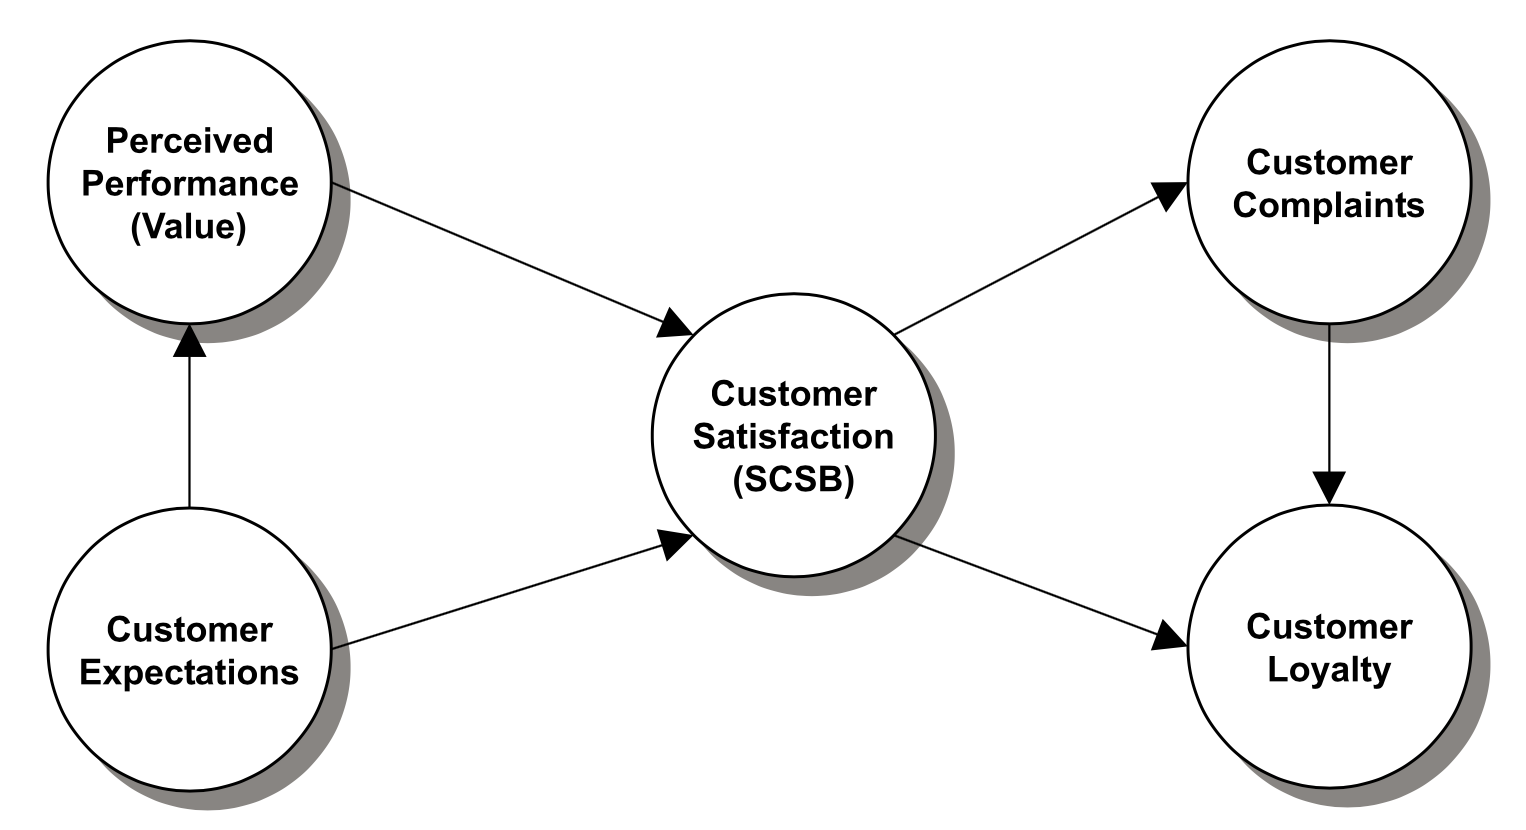
\includegraphics[width=1.0\textwidth]{img/scsb.png}
	\caption{Model used for Swedish Customer Satisfaction barometer \cite{fornell1992national}}
	\label{fig:scsb}
\end{figure} 

Although the model experienced some critics in the following years as further national Customer Satisfaction surveys were deployed they all were based on and inspired by the original ideas of the swedish model. A more enhanced analysis of the existing model approaches was done by \cite{johnson2001evolution}. As a result of the derived strengths and weaknesses from different Customer Satisfaction barometer models, they proposed a new model which was used as the base model by this thesis to build its further empirical work on. The model is visualized in figure \ref{fig:satisfactionModel}. Each of the different parts will be described briefly to get an overview on the essential components and their relationships and adaptations in contrast to the initial base model, namely the SCSB, as well as the limitations drawn by the author regarding the work in this thesis. 

\begin{figure}
	\centering
	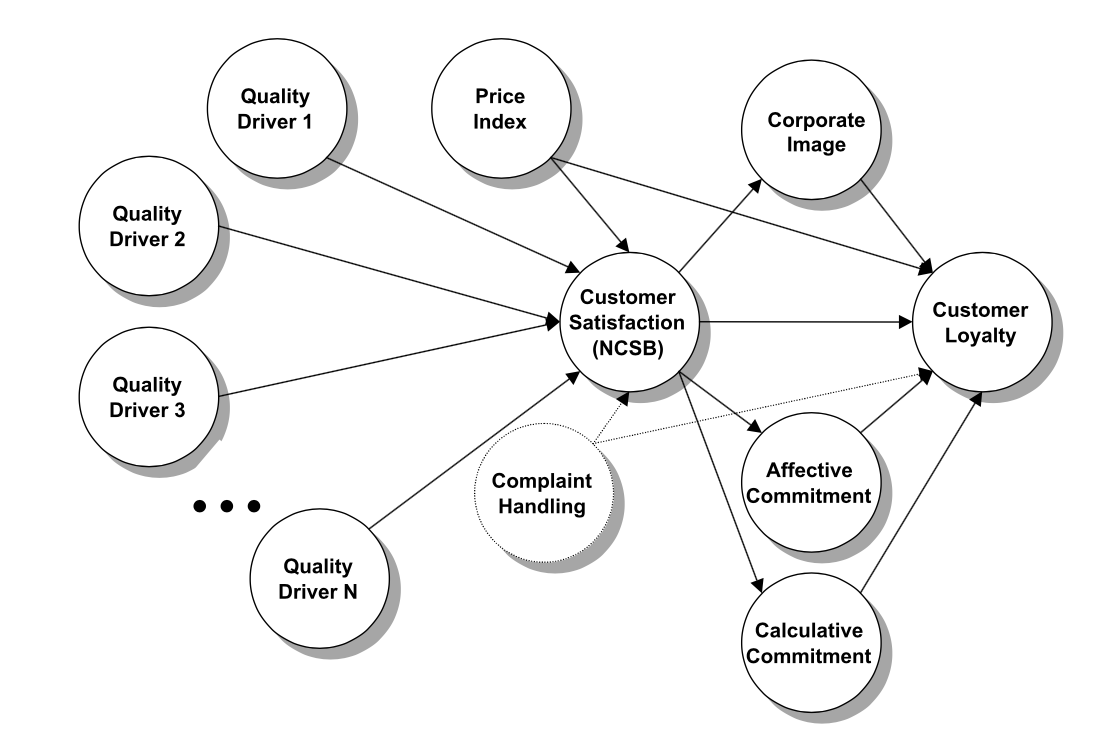
\includegraphics[width=1.0\textwidth]{img/custSatisfaction.png}
	\caption{Customer satisfaction model proposed by \cite{johnson2001evolution}}
	\label{fig:satisfactionModel}
\end{figure} 

The first difference when comparing the latter proposed model with the SCSB is the role of customer expectations. Since satisfaction has to be observed over a longer time period, expectations get adapted throughout repeated consumption experience as well. More emphasis is put on the quality delivered by the product and the expectations are considered to be evaluated regularly due to this quality. These statements can be supported among several industries including the communications sector which the author considers as similar to the field the case study of this thesis operates in \cite{johnson1996expectations} \cite{fornell1996american}. Despite that fact the author does not completely agree with these findings to remove the term "customer expectations" totally. Instead of the expectation parameter, 1-n perceived quality criterion are predictors for Customer Satisfaction. Next to the quality drivers the perceived price for the provided product quality plays a role as well. The third satisfaction driver illustrated in this model is complaint handling. Due to evolvement of customer support services, customer complaints cannot be stated as simple negative outcome of Customer Satisfaction. More specifically support influences emotions either negatively or positively and as a consequence is a direct predictor of satisfaction. It may even has an impact on repurchase behavior of customers which explains the direct relationship to customer loyalty \cite{johnson2001evolution}. 

The three remaining components have not yet been mentioned explicitly regarding their role in the customer satisfaction construct. All of them are directly influenced by the outcome of Customer Satisfaction while mediating the loyalty parameter. The corporate image, or sometimes called brand reputation, indicates how popular and known a company is in the public. Consumption experiences of a customer affects the corporate image in a certain direction as well. According to a study of \cite{hussain2015service} a dissatisfied customer tells on average nine other people about negative experiences which can heavily affect loyalty. Although the corporate image is part of the model it will not be discussed or used further in the empirical work of this thesis because it can not be measured by usage behavior and quality data collected by IT systems. Similarly the affective- and calculative commitment mediate parts of the effect of Customer Satisfaction on loyalty. While the affective component resides on the emotional side and mainly relates to trust with regard to a brand, the calculative component is more rational in terms of costs. (e.g.: costs for a customer to cancel a relationship and switch to a competitor) \cite{johnson2001evolution} Both components were mentioned for the purpose of completeness but are not elaborated in more detail since they cannot be represented in the available data of the case study. 

\section{Measurement of Customer Satisfaction}
As the reader got an overview on the parts and influential factors of Customer Satisfaction, the next step is to look at possibilities to transform the defined model properties to quantitative measurements. On the one hand this thesis evaluated survey based measurements and looked in more detail on different types and their performance. On the other hand it was tried to find approaches to measure Customer Satisfaction without survey data based on implicit satisfaction representing patterns in huge data sets. 

\subsection{Theories about Customer Satisfaction determination}
\label{ssec:custSatTheories}
Although there has been a lot of research regarding a formal definition of Customer Satisfaction, less papers were published on how satisfaction can be quantitatively measured. One approach based on the original expectancy-performance disconfirmation model was to design a survey asking customers how they would rate

\begin{itemize}
	\item their expectations regarding to a set of chosen dimensions before usage and
	\item the perceived performance and quality of the product with regard to the same set of dimensions \cite{prakash1983reliability}.
\end{itemize}

This approach seems to be promising as it respects the originally identified and well researched Customer Satisfaction model. However, it brings problems regarding the expectation parameter with it and thus make it inappropriate for this thesis. Firstly, expectations can hardly be measured unbiased since they get evaluated by the customer alongside with the perceived quality in case of using one satisfaction survey \cite{getty1995relationship}. As outlined in \ref{custSatisfactionDefinition} the proposed model is based on cumulative satisfaction evaluation which yields regular adaptations on what a customer expect from a product. Asking customers about their expectations, with regard to a specific set of product dimensions, explicitly before usage neither makes any sense from a business perspective of Tractive nor is the author able to initiate a process to collect such data. Secondly, measuring customer expectations turns out to be difficult as people tend to rate their expectations, if they have to state them explicitly, very high on average \cite{babakus1992empirical}. As a consequence the uniform overrating of customers expectations will not provide any extra information in assessing customer satisfaction from a survey. As last point in the considerations regarding this approach, the validity of stated expectations has to be questioned since customers often do not have specific expectations before using a product. A dominant reason for this phenomenon is especially observed in software products or services due to its variable and intangible nature. Following, it was found that if customer expectations cannot be formed well, the expectancy-performance disconfirmation metric looses its worth \cite{halstead1994multisource}. 

The mentioned arguments and following impracticality required the need for further research on suitable approaches to assess Customer Satisfaction. In contrast to the research branch which insists on the importance of considering expectations in measurement, there has also been research experience in favoring the perceived performance or, depending on the Customer Satisfaction model, the perceived value \cite{yuksel1998customer}. Based on the mentioned disadvantages in assessing expectations it is claimed that perceived performance reflects the subjective response and emotional feeling as outcome of a consumption experience and thus is seen as the major source in steering the satisfaction value into a particular direction \cite{halstead1994multisource} \cite{cronin1992measuring}. Although perceived performance alone is claimed to perform well as measurement indicator for Customer Satisfaction, a lot of different data dimensions tie together an overall quality or performance. Depending on the dataset the collected parts can correlate in a certain way, be independent, redundant or differ by their importance in contributing to the overall satisfaction. Thus, taking the importance of quality indicators into account can be crucial in determining why a customer might be more satisfied than a similar one \cite{barsky1992customer}. Based on these findings and results in past research this thesis follows, with regard to the case study, the hypothesis that collected usage behavior data is especially of interest if related to quality and performance of the product respectively offered service. With a view to the empirical work, the available data at Tractive provides enough quality and performance indicators. This data is collected transactional-oriented with the customers usage of the Tractive GPS products and can be used when following this measurement approach. 

\subsection{Quantitative metrics for classification of satisfaction outcome}
Before being able to elaborate on the taxonomy of statistical- and data-mining related methods, the open question, on how a Customers satisfaction feeling can be measured reliably by quantitative metrics, has to be answered. 

In order to be able to reveal reliable patterns and influencing factors in quality and performance data when executing analysis methods, some sample satisfaction data from customers is needed. Otherwise no educated comparisons of results are possible and they would only be wild guesses. Due to the complexity of building a customers attitude towards a product, the preferred way is to collect quantitative data representing satisfaction by a survey \cite{yuksel1998customer} \cite{hayes1998measuring}. Especially the software industry is a sector where it is hard to classify a customers satisfaction based on objective data implicitly gathered by the systems without asking any person \cite{hayes1998measuring}. However, conducting a Customer Satisfaction survey turns to be a difficult task. On the one hand it should support later analysis by enough sample data, while on the other hand it should also collect enough useful satisfaction measurements from customers to derive expressive results \cite{sauermann2013increasing}. 

There have been different opinions in research on how a Customer Satisfaction survey should be structured and how comprehensive the content has to be. \cite{hayes1998measuring} proposed a process where all quality dimensions of a product, considered as important by the survey issuer, should be collected since this promises to provide a complete view on the whole product separated by its characteristics. The author of this thesis sees it differently because the research objective is to reason about an overall satisfaction of customers without knowing any subjective opinion from them. Plus, response rates will decrease the more items a survey contains. The essential priorities for the researcher is first, collecting many survey answers to have a bigger chance in finding significant patterns and learn more reliably from the data and second, keeping understandability of results rather simple \cite{sauermann2013increasing}. In dependence on the scarce resources of businesses in very competitive markets, as the software industry for instance, approaches and outcomes of research developed into the direction of making surveys much shorter but with wisely chosen questions which are useful to reason about loyalty of customers which in turn is strongly connected to profit \cite{reichheld2003one}. When designing a Customer Satisfaction survey to collect sample data for the analysis part, these latter ideas were taken under consideration. 

\section{Taxonomy of methods for behavioral analysis and satisfaction prediction}
The research work in finding and evaluating different analysis methods and prediction approaches is described in this section. The following paragraphs will outline existing process models and approaches which were either already tried and evaluated in the extended field of Customer Satisfaction or may be otherwise relevant and suitable for the implementation part of this thesis. 

\subsection{Overview on an analysis approach}
Before thinking about suitable approaches and their implementation, it is important to clearly state the goal of the analysis and data planned to use in order to reach the goal. The analysis data contains the information necessary to perform the concrete analysis and should support reaching the desired goal. In this generic picture, it does not matter how this data got collected, its representation and how it can technically be extracted and queried. In first place it is important to ensure that this data is available and relevant. On the opposite end of the process one has to formulate the analysis goal which guides the procedure and always has to be kept in mind as the ultimate question which should be answered. Thus, the analysis goal is limited to yet unknown properties and information which cannot be directly queried from available data. Specifying analysis- data and goal yields an analysis problem to be solved. \cite{neckel2015} \cite{knobloch2000data}. The process is illustrated in figure \ref{fig:analysisProcess}.

\begin{figure}
	\centering
	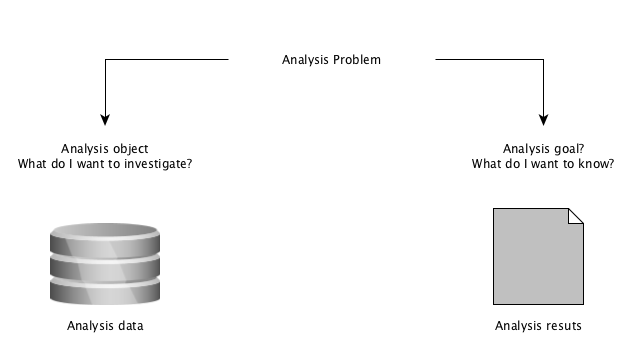
\includegraphics[width=1.0\textwidth]{img/analysis.png}
	\caption{Analysis process \cite{neckel2015}}
	\label{fig:analysisProcess}
\end{figure} 

When having specified an analysis problem, the hard part of solving it with a suitable analysis approach is still pending. It is not limited to the analysis algorithms itself but rather involves a whole process of selecting, preparing- and finally analyzing the data in a way to satisfy the formulated goal. 

Basically, when analyzing customer related data and its effect on a business, it has to be distinguished between two major analysis categories, namely the top-down (hypotheses-driven)- and the bottom-up (data-driven) approach \cite{neckel2015}. As this thesis followed these two approaches on the way to answer the stated research question, the upcoming sections will shed more light onto them and their appliance in existing research projects.

\subsection{Top-down analysis approach}
\label{ssec:topDown}
The objective of a top-down analysis is to get an overview on the initially selected data and be able to reason about the influence of particular attributes. In order to perform a top-down analysis it is required to have a better knowledge of the data to be analyzed. The reason is that this type of analysis is based on an explicitly formulated hypothesis which should be proved and as a result verified or falsified. In essence, such an analysis usually starts with well-defined assumptions. In terms of Customer Satisfaction analysis, a domain expert supposes influential factors and knows which data is representative enough. However, it is unknown whether he or she is right at all, how strong such a particular relationship in reality is and which direction the potential predictor correlates with the target variable. Those are then the resulting questions stated explicitly with hypotheses and to be answered by a top-down analysis approach. Due to the nature, it heavily relies on statistical methods to prove the formulated hypotheses. This involves different kinds of statistical tests depending on the type of data required to execute the analysis \cite{neckel2015}. Published research resources about top-down analysis in the field of Customer Satisfaction are rare. The main purpose turned out to be inductive statistical analysis. 

\subsubsection{Suitable statistical tests}
The main purpose of a statistical analysis in the top-down approach is making a statement about the behavior of a population based on a representative sample. Such an analysis is also called Inductive statistics. Since it cannot be known upfront how well the selected sample actually represents the population, the probability of a particular result with regard to prediction of the actual outcome gets quantified. This is usually done via a confidence interval, indicating an allowed error $\alpha$ within a hypothesis is proven to be valid \cite{oestreich2009keine}. Depending on the type of data, an appropriate statistical test should be chosen. Regarding the empirical work in this thesis, two types of sample data will be relevant in the top-down approach, namely categorical- and continuous numerical data. 

As the categorical data to be considered in the very first analysis will only be of binary type, the Fisher's exact test turned out to be the best choice to analyze a potential statistical significant difference between the two categorical groups under consideration. Details about this test can be found in \cite{fishers1992}. 

In order to compare data rows consisting of numerical values which do not have an order to allow for directly ranking  them, the popular Pearson correlation coefficient was leveraged by this thesis. It is a quite powerful solution to analyze a linear relationship between numerical data rows and also indicates its direction and strength. Although this method has the disadvantage that it cannot reason about any non-linear relationship, the author expected that the correlation behaves in a linear manner in order to identify drivers of Customer Satisfaction. Since the correlation coefficient is only a point estimation, there is need for an inductive measurement to reason about the population. Under the assumption that both data rows are at least asymptotic normal distributed, there is the possibility to calculate a confidence interval for the correlation coefficient and in turn execute a statistical test to verify a hypothesis. This test is called Pearson's product moment correlation coefficient. If the value confidence interval does not include the value $0.0$, a statistical significant result can be followed \cite{lee1988thirteen} \cite{artusi2002bravais}. 

\subsubsection{Selecting data samples}
Despite the fact that the scope of data to be analyzed is specified by a given hypothesis, statistics were found to react sensitively with regard to sample sizes and quality of data. While the representativeness of a selected sample is left to the particular use case, interesting research results were proposed with regard to the sample size to choose. One has to keep in mind that the sample size can heavily influence the power of analysis methods as a statistical significance alone is not expressive enough. One also has to put emphasize on the so called clinical relevance which originates from inductive statistical analysis in the medical field \cite{campbell1995estimating}. This relevance value defines the minimum effect which should be detected as for instance in case of categorical data between the control and treatment group \cite{kadam2010sample}. In case of correlation analysis, this would be the minimum coefficient considered as relevant for indicating a sufficient linear relationship \cite{moinester2014sample}. It is important to notice that in order to prove for a smaller effect size, which is equal to a small confidence interval, the sample size has to be larger. In contrast, a large effect size, which equals a bigger confidence interval, reduces the required sample size. In addition to the minimum effect size, the $\alpha$-error, indicating the maximum allowed false-positive rate and the $\beta$-error, indicating the false-negative rate, are necessary input parameters to estimate an optimal sample size \cite{kadam2010sample}.

\subsection{Bottom-up analysis approach}
\label{ssec:bottomUp}
In contrast to the top-down analysis approach, the bottom-up (also known as data-driven approach) does not involve explicit hypotheses to prove. Instead, the questions of a data analyst in this case start very general and initial assumptions are vague. Researchers for instance can use the stated research question as initial analysis goal. As a result, these characteristics make the whole analysis approach much more complex as there are no upfront decisions made about specific datasets to be used in order to answer the question respectively to solve the analysis goal. This type of analysis can also be interpreted as searching in a huge data jungle where several intermediate analysis problems have to be solved before being able to solve the original analysis problem. After solving such an intermediate challenge, one gathers more insights in the data and new patterns are revealed over time \ref{neckel2015} \cite{fayyad1996data}. Research in this are has become highly competitive and different buzzwords started to raise attention to a broad audience. To prevent confusion in the upcoming sections, the author decided to briefly explain the essential terms. Following listing names the terms as they will be used in the rest of this thesis. The interpretations are based on the findings from \cite{fayyad1996data}. 

\begin{itemize}
	\item Knowledge Discovery in Databases (KDD): In abstract terms KDD can be seen as the comprehensive process to gather some useful knowledge from collected data in a database. With regard to the prediction of Customer Satisfaction, it can be interpreted as the procedure starting with processing of all customer related data till building a model which allows predicting whether a customer is (dis)satisfied.
	\item Data mining: This involves the actual algorithms to find and extract the desired information from the prepared data. In essence, it is merely one step in the knowledge discovery process, namely the prediction step with regard to this thesis. 
	\item Machine learning: It is a very controversial term as it is used differently in practice. In research however it describes techniques and algorithms to learn from data and as a result follow statements for related but unknown data (i.e. derive new knowledge). Machine learning is therefore a methodology applied in data mining. 
\end{itemize}

A comprehensive KDD process is illustrated in figure \ref{fig:kddProcess}.

\begin{figure}
	\centering
	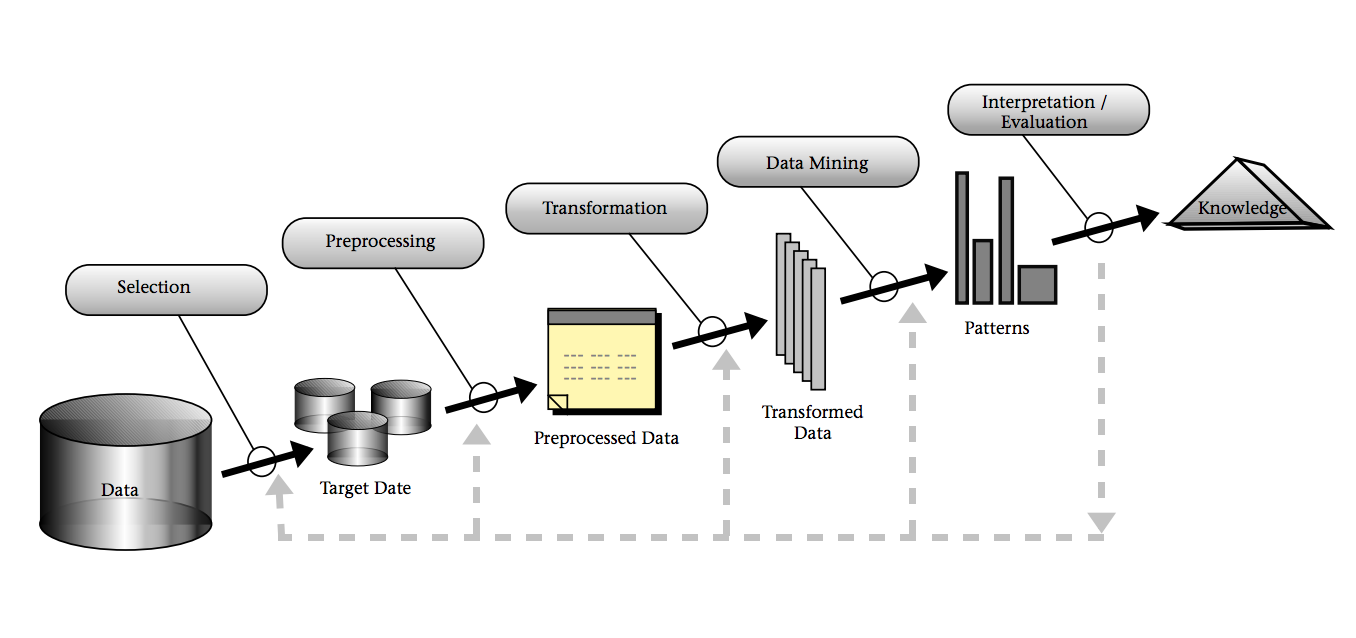
\includegraphics[width=1.0\textwidth]{img/kdd.png}
	\caption{Big picture of a KDD process \cite{fayyad1996data}}
	\label{fig:kddProcess}
\end{figure} 

Understanding and predicting customers behavior is considered valuable for businesses and therefore a lot of research has been done in mining customer data to gain interesting insights and take the right decision before a competitor does so \cite{Ngai2009}. Since a major part of the empirical work in this thesis dealt with finding behavioral patterns in customer usage data, different existing methods were studied and evaluated. The following sections provide an overview on the steps of a suitable bottom-up approach and focuses on relevant methods with regard to the implementation.

\subsection{Pre-analysis work}
As extracted from the literature review by \cite{Ngai2009}, dozens of research papers introducing data mining approaches to solve particular business problems in dealing with customers have already been published. However, no matter how powerful and sophisticated those proposed methods are, none of them will work successfully on unwisely chosen, invalid or bad quality data. This fact emphasizes the importance of preprocessing and preparing data accordingly to increase the chance of retrieving meaningful analysis results \cite{neckel2015} \cite{knobloch2000data}. The pre-analysis can be broadly divided into following sub categories:

\begin{itemize}
	\item Selection of data
	\item Preprocessing of data
	\item Transformation of data
\end{itemize}

The following sections \ref{sssec:selectionData}, \ref{sssec:explorationData} and \ref{sssec:manipulationData} will provide a more detailed overview on these pre-analysis categories and should give the reader an understanding of the involved tasks. 

\subsubsection{Selection of data}
\label{sssec:selectionData}
Depending on the type and goal of analysis tasks, the whole database management system of the business should be searched for relevant data collections. In order to optimize this raw data selection process, quality criterion should be determined to prevent choosing irrelevant or invalid data at an early stage \cite{mozer2000predicting} \cite{fayyad1996data}. In terms of Customer Satisfaction analysis, focus has to be put on data collections indicating quality and performance dimension resulting from usage behavior, as this was identified as reliable measurement source in section \ref{ssec:custSatTheories}. Existing approaches belonging to the context of this thesis, like \cite{mozer2000predicting}, \cite{meinzer2016can} or \cite{zhao2005customer} insist that identifying relevant data sources upfront by domain experts makes the overall process better as only a subset of available customer data has to be analyzed and this saves time. A not negligible part in the selection stage is the orientation of data. Research talks about transactional-oriented data in case it results from operative application. Although this transactional data provides opportunity for intensive analyses, it is not always on the desired level of detail. Then it makes more sense to use data which is stored in an analytical oriented format and thus provides a meaningful aggregated view on interesting parts of a data collection \cite{neckel2015}. 

\subsubsection{Preprocessing of data}
\label{sssec:explorationData}
After limiting the number of data sources, a crucial step is to explore the collected data in order to reason about quality and find potential weaknesses- and problems one has to tackle before moving on to the next step. What was found out during literature research is the fact that despite the rather huge amount of publications regarding technical implementation of knowledge discovery and data mining methods in the customer management area, few put emphasis on preprocessing of data. The effort taken by many authors on particular stages in the preprocessing pipeline, as illustrated in figure \ref{fig:kddProcess}, emphasizes the importance of preparing data before applying specific data mining techniques, like classification, on it. The optimal path through the preprocessing pipeline is hard and cannot be generalized as it turns out to be different for each dataset. Due to the heterogeneous nature of usage behavior data, this step has major influence on the prediction outcome of this thesis research \cite{fayyad1996data}. 

In large customer generated datasets it is common that some data attributes may be important on the one hand but provide unreliable, erroneous or missing information among several data observations on the other hand. Thus data cleaning was identified as essential part in the preprocessing step \cite{fayyad1996data}. Especially a well defined procedure for handling missing attribute values among data observations has been a desire for a long time. The work of \cite{batista2003analysis} compares methods for handling missing attribute values for data observations with each other and analyzes both strengths weaknesses of them. It was found out that one has to get a clear understanding on the reasons why certain attribute values are missing. Three different categories, namely MCAR (Missing Completely At Random), MAR (Missing At Random) and NMAR (Not Missing At Random) can be differentiated according to \cite{little2014statistical}. 

Completely random missing data does not allow to find any predicting variable. Neither known values of the affected instance nor any other missing value among data observations has an impact. In this case any of the available treatment methods leads to unbiased results. In essence this means that it does not matter which method is chosen. The second type, namely NMAR, deals with missing data resulting from unobserved characteristics. This could for instance affect the outcome of interviews with persons who keep some secrets for them and therefore introduce missing data. This type is not considered as relevant in the customer behavior data as customers, frankly said, cannot hide details collected due to their usage behavior. As a consequence data when collected automatically by a computer system mostly falls into the MAR category \cite{donders2006gentle}. It was determined that neither simply discarding particular instances with missing values among attributes nor totally ignoring a subset of attributes with too many missing values are favorable techniques for this type of data. Different methods to replace missing values, as evaluated by \cite{donders2006gentle} and \cite{batista2003analysis}, were analyzed in the literature review of this thesis and serve as base for data cleaning work in the implementation part of this thesis. Although not promised as the most reliable method in literature, methods like imputing missing values with mean and mode are, due to its simplicity, popular in the area of machine learning. However, depending on the nature of data it is recommended to take an eye on more sophisticated imputation approaches \cite{batista2003analysis}. 
\newline
\newline
The second essential thing to have an eye on when preprocessing the extracted raw data set is the potentially unfavorable distribution of satisfaction levels. Literature research showed that many existing data mining approaches, dealing with classification, had to actively combat this problem in order to increase accuracy of their algorithms in the prediction process later on. Domains affected heavily by this problem are for instance medicine, when it comes to diagnosis of diseases, or fraud detection algorithms in payment systems \cite{chawla2004special}. These domains can sometimes experience imbalances as extreme as 99\% of a majority- against 1\% of the minority class \cite{he2009learning}. The identified difficulties resulting from such extreme imbalances are on the one hand algorithms, which try to learn from this data, and on the other hand misleading accuracy results presented to the researcher. A typical classification algorithm is well advised to choose the majority class as a prediction result and does not really consider the minority class at all. As a result this leads to an accuracy of correctly classified instances close to 100\% but is totally ignoring the minority class. Such a view on the results turns out to be absolutely worthless \cite{chawla2002smote} \cite{kubat1997addressing}. 
\newline
\newline
As a consequence different solutions have been proposed over the last decade to alleviate the problem and find better performance measures to evaluate classification algorithms. For imbalance problems, sampling mechanisms with the goal of artificially creating balance between the classes were developed. Due to the rather high number of researchers trying to optimize their solutions as well as the amount of different approaches proposed, the sampling mechanisms became a controversial topic. Although working quite well when evaluating them in training, some produced completely different results in practice. This led to an increased number of authors who started to put their hands on the algorithms itself to introduce penalties for wrong classification of data observations and thus steer the algorithm in the correct direction \cite{chawla2004special}. As mentioned by many authors, simply choosing the classification accuracy as first-class measure is definitely not preferred in cases of imbalance. Over the years especially the ROC (Receiver-Operating-Curve) has established as favorable performance measure \cite{fawcett2006introduction}. Although it is not expected that there is an extreme imbalance between satisfied and dissatisfied customers, this step in preprocessing attracted attention to the author as it turned out to be a critical point in the area of classification problems.

\subsubsection{Transformation of data}
\label{sssec:manipulationData}
After having revisited the selected data, brought it into the desired format and prepared it by applying and tuning chosen preprocessing approaches, a final step before moving on to the actual prediction task is data transformation. A general applicable task within this category is feature scaling also known as feature normalization. The purpose hereby is to overcome the problem of different types and units of data as it is typical for datasets which are topic of data mining. Due to the rather large amount and heterogeneity of features in related research projects as \cite{mozer2000predicting}, \cite{meinzer2016can} or \cite{zhao2005customer}, scaling features to a unit scale is considered a duty in order to ensure that classification algorithms take right decisions when learning from provided data. Most popular and widely used scaling mechanisms are the linear scaling to a unit interval range and the standardization to a normal distribution with zero mean and standard deviation of one. Following are the mathematical equations \cite{aksoy2001feature}. 

Linear scaling unit: $\tilde{x} = \frac{x - min}{max - min}$

Whereby x is the value of a particular data observation for a specific feature, min and max is the minimum respectively maximum existing value for this feature among all data observations. 

Standardization to normal distribution: $\hat{x} = \frac{x - \mu}{\sigma}$

In the equation above $\mu$ is the mean value of the feature currently looked at and $\sigma$ is its standard deviation.

As it can be seen from the equations, these scaling mechanisms are quite trivial but turn out to be an effective strategy to make working with different distance measures in data mining possible and correct.

% TODO: Feature engineering should be mentioned somewhere
\subsection{Predicting satisfaction by leveraging classification algorithms}
When the data is finally in the required representation and preprocessed in a way to have eliminated as many flaws in the data as possible, the actual data mining work can be started. Therefore this section deals with the appliance of a machine learning algorithm which fits best to the prepared customer data set. There has already been lot of research in predicting customer churn as this is an interesting management topic in various industry sectors. As its prediction outcome is binary (i.e. churn or not churn) a classification algorithm turned out to fit best \cite{vafeiadis2015comparison} \cite{xie2009customer}. Although Customer Satisfaction is on a higher abstraction level and more difficult to grasp, features used for churn prediction show similarities to the potential features used for overall satisfaction prediction. It thus served as a good starting point for getting an understanding which classification techniques seem promising. Literature research showed that finding an outstanding classification algorithm cannot be guaranteed for this domain in general. More specifically to Customer Satisfaction tied material from \cite{mozer2000predicting} and \cite{meinzer2016can} did not lead to clear results regarding algorithm choice. However, it can be derived that decision trees and SVM (Support Vector Machine) were evaluated as well performing algorithms for such a type of problem \cite{vafeiadis2015comparison}, \cite{xie2009customer}, \cite{mozer2000predicting}, \cite{meinzer2016can}. Therefore the implementation work of this thesis mainly concentrated on these algorithms which will be briefly introduced in the following sections.

\subsubsection{Decision trees}
Decision tree algorithms are a one of the most mature techniques available in machine learning. They are considered as quite popular and are often used in practice since they are pretty easy to understand, well-performing across different data mining challenges and much faster than other techniques with high runtime complexity. Per definition a decision tree algorithms tries to find an optimal way to hierarchically split the labeled training input data based on expressive features in order to build a model of rules which best represent the target variable. This procedure is done recursively whereby for each split all available features get considered, the one which promises the best separation regarding the class label will be taken for the current split and in turn represents the according split rule. This model can then subsequently be applied on a real dataset to predict the class of data observations following the best path defined by the rules built earlier \cite{linoff2011data}. 

Although the basic principle of a decision tree is fixed, different implementations, which mainly differ in the way of determining the optimal split in each iteration, have been proposed over the last years. As a particularly powerful measurement regarding an optimal selection of a feature as well as a split rule, the concept of Information Gain respectively entropy reduction has emerged. The technique is used in the nowadays popular C4.5 decision tree implementation developed by Ross Quinlan. It is the concrete base algorithm used in the empirical work. 

A promising modification regarding classification accuracy is the Random Forest algorithm proposed by Leo Breiman in 2001. Instead of finding the best split in each iteration, a defined number of feature subsets is taken. Several trees for the best splits found among those subsets get constructed. The best combination is subsequently obtained by a voting mechanism. 

% TODO: Find out in which degree of detail these mature algorithms have to be described. 

